%Esta plantilla la usamos desde el 2018, si tienen alguna obervación pra mejorar, por favor mándenme un correo
% vvazquez@fcfm.buap.mx

\documentclass{siep}
\usepackage[spanish]{babel}
\usepackage[utf8]{inputenc}
\bibliographystyle{dcu}
\usepackage{cite}
\spanishdecimal{.}

\title[T\'itulo Corto Aqu\'i]{Plantilla para elaborar su ponencia en extenso}

\author[ad1][ad2]{Nombre Apellidos}
\author[ad1][]{Second AUTHOR}
\author[ad1][ad2]{Third AUTHOR}
\author[ad2][]{Fourth AUTHOR}


\correspondingauthor{Second AUTHOR} %aquí se determina al autor de correspondencia

\address[ad1]{Institute of xxx xxx xxx xxx\\ University of xxx xxx, Address xxx xxx xx xxx xxx\\ e-mail: \url{email1, email2, email3}}
\address[ad2]{Institute of xxx xxx xxx xxx\\ University of xxx xxx, Address xxx xxx xx xxx xxx\\ e-mail: \url{email4}}

%\authors{First name LAST NAME \!$^{a}$, Second AUTHOR \!$^{a, b,}$\thanks{Corresponding author. \newline The authors are listed in}. \,\,,\\ Third AUTHOR \!$^{b}$}
%\addresses{$^{a}$\! Insti-ute of xxx xxx xxx xxx\\ University of xxx xxx, Address xxx xxx xx xxx xxx\\ e-mail: \url{xxx xx xxx}\\\medskip $^{b}$\! Second affiliation}

\Runauthors{Primer autor \it{et al.}} %Aquí puede ponerse el nombre del primer autor et al
%\Runauthors{J. Doe}
%\Runauthors{J. Doe and M. John}

%PLEASE DO NOT MODIFY OR REMOVE THESE!
%\Year{}
%\Vol{}
%\No{}
%\Startpage{}
%\Endpage{}
%\DOI{}
%\Received{}
%\Revised{}
%\Rerevised{}
%\Accepted{}
%\bibliographystyle{dcu}

\begin{document}
\begin{abstract}
Aqu\'i va el resumen del trabajo.
\end{abstract}

\begin{keywords}
keyword 1, keyword 2, \dots, keyword 5. Please provide a few keywords (3--5) and keep them specific.
\end{keywords}
\maketitle

\section{Introduction}
Algunas paqueter\'ias son necsarias para usar esta plantilla: \verb+times+, \verb+amsmath+, \verb+amssymb+, \verb+color+, \verb+graphicx+, \verb+caption2+ with the option \verb+hang+, \verb+harvard+ with the options \verb+dcucite+ and \verb+abbr+.


\section{El t\'itulo}

Por favor que no sea demasiado extenso.

\medskip


\subsection{Sobre los autores}
Notar que cada autor puede estar afiliado a lo m\'as en dos instituciones

\medskip
\noindent {\small \verb+\author[ad1][ad2]{Nombre}+}.

\medskip\noindent
Si alg\'un autor s\'olo pertenece a una instituci\'on, el segundo par de corchetes debe estar vac\'io.


\medskip
\noindent {\small \verb+\author[ad1][]{Author's NAME}+}.


\section{Elementos flotantes}

Para incluir elementos flotantes como las im\'agenes, se pueden seguir los siguientes ejemplos.

\begin{figure}[!b]
 \centering
  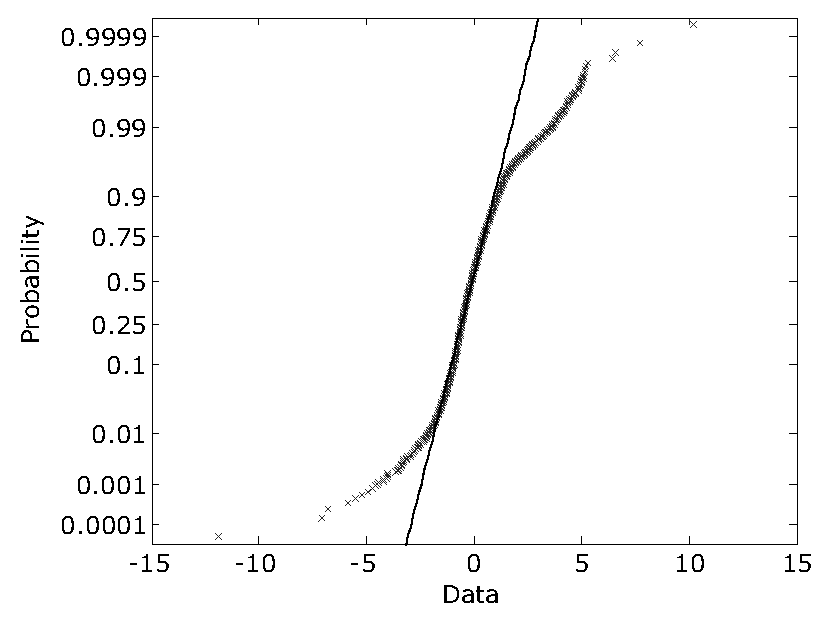
\includegraphics[width=0.45\textwidth]{fig1}
 \caption{Figure example.}
  \label{fig1}
\end{figure}


%%%%este ejemplo muestra c\'omo poner dos im\'agenes al mismo nivek en las dos columnas

\begin{figure*}[!t]
 \centering
  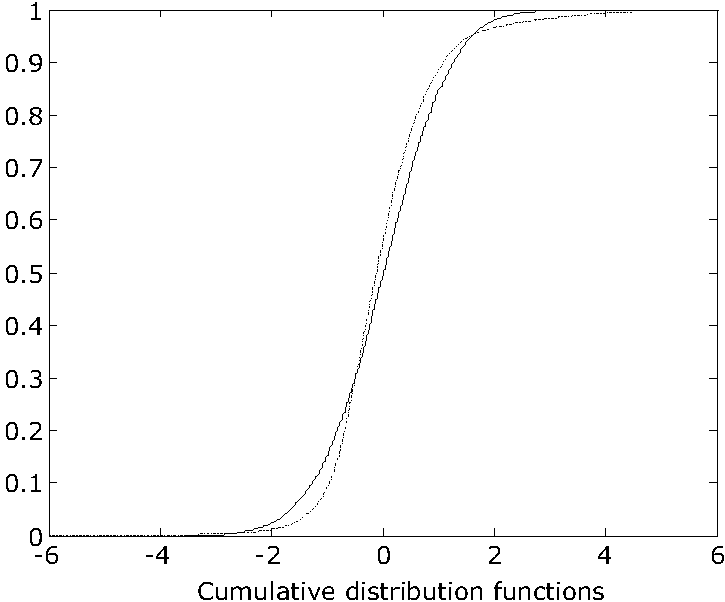
\includegraphics[width=0.40\textwidth]{fig2a}\hspace{0.5cm}
  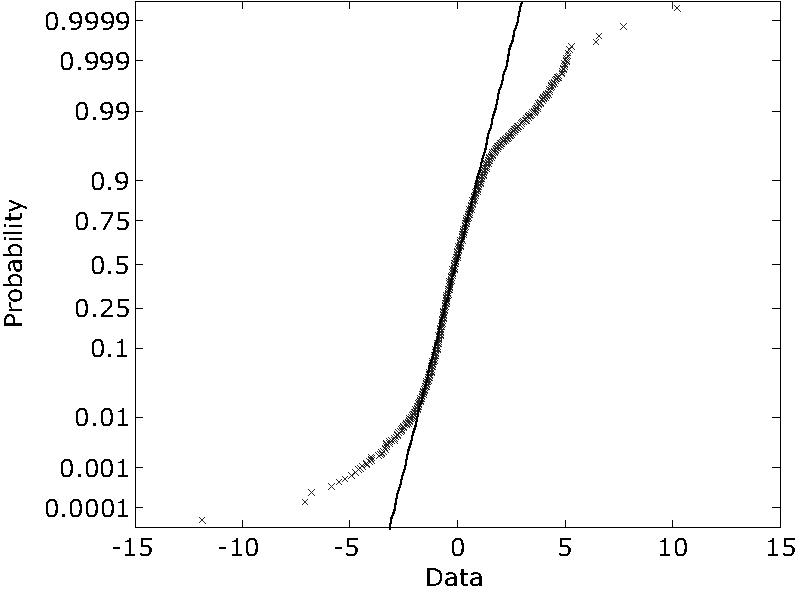
\includegraphics[width=0.45\textwidth]{fig2b}\\
  (a)\hspace{8cm}(b)
  \caption{Sample figure: the first graph (a), the second graph (b).}
  \label{fig2}
\end{figure*}


\subsection{El ejemplo en acci\'on}
Figures are defined in a standard manner, e.g.,
{\small \begin{verbatim}
\begin{figure}[!b]
 \centering
 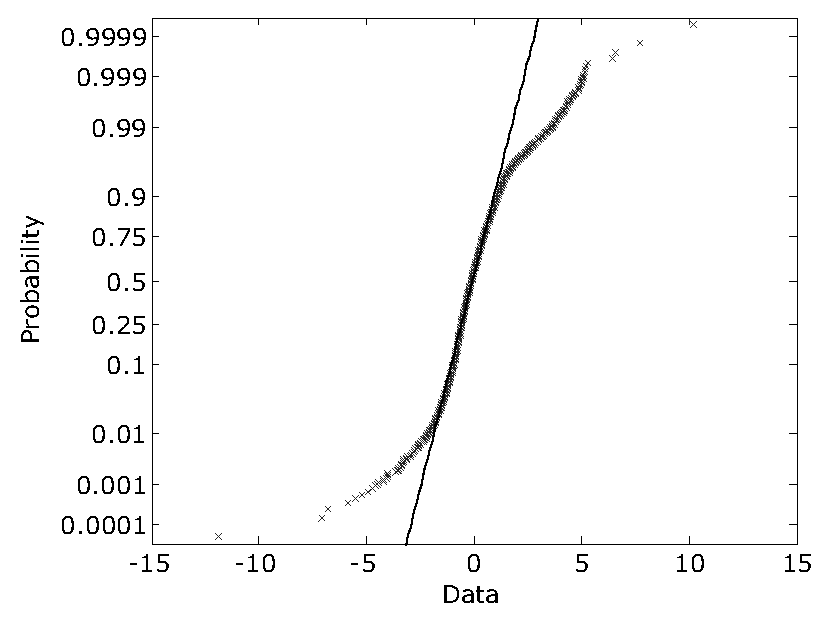
\includegraphics[width=0.45\textwidth]
 {fig1}
 \caption{Figure example.}
 \label{fig1}
\end{figure}.
\end{verbatim}}


{\small \begin{verbatim}
\begin{figure*}[!t]
 \centering
 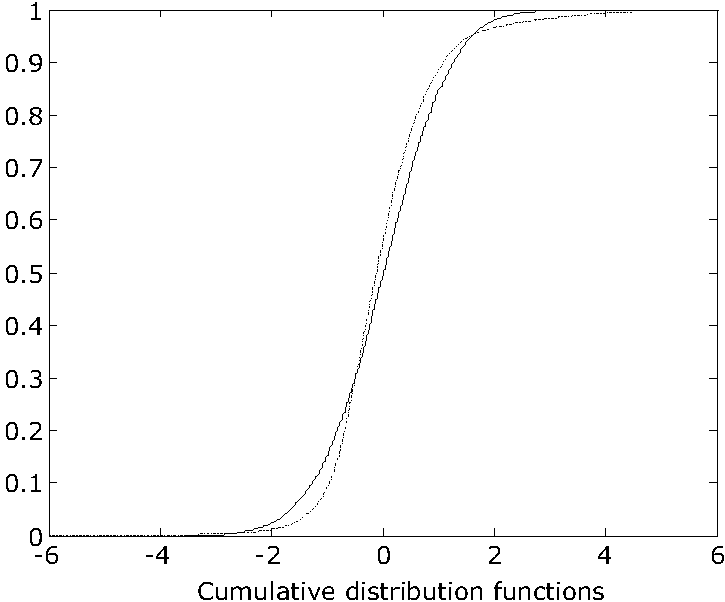
\includegraphics[width=0.405\textwidth]
 {fig2a}\hspace{0.5cm}
 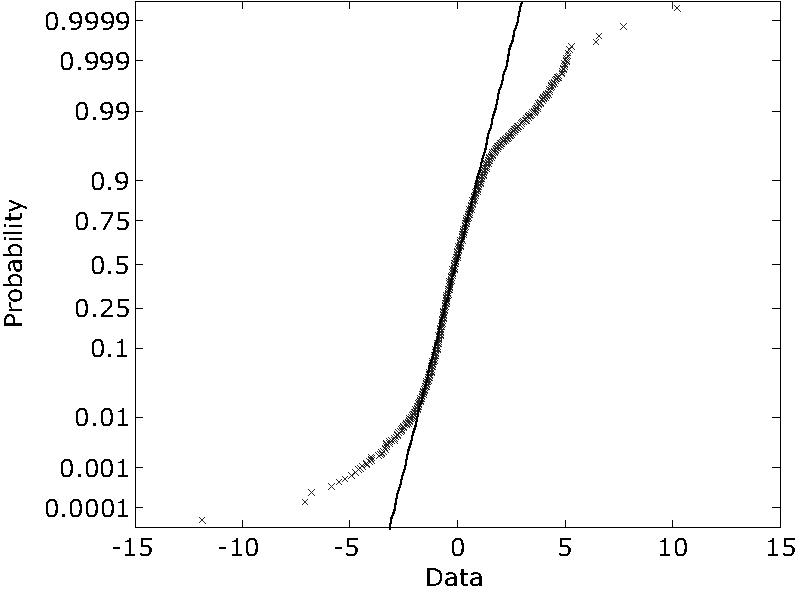
\includegraphics[width=0.45\textwidth]
 {fig2b}\\
 (a)\hspace{7cm}(b)
 \caption{Sample figure: the first
 graph (a), the second graph (b).}
 \label{fig2}
\end{figure*}.
\end{verbatim}}

When referring to figures, the abbreviation ``Fig.'' should be used. It is also advisable to clearly name the graphic files and their labels, e.g., \emph{fig1, fig2a, fig2b}, etc.
\subsection{Tablas}
%
Este es un ejemplo para hacer tablas
%
{\small\begin{verbatim}
\begin{table}[!b]
 \centering
 \caption{Table example.}
 \label{table1}
 \begin{tabular}{|c|c|c|}
  \hline
  Algorithm & Performance [\%]& Calc. time
  [s]\\\hline\hline
  gradient & 95 & 100\\
  stochastic & 97 & 80\\
  evolutionary & 99 & 500\\\hline
 \end{tabular}
\end{table}
\end{verbatim}}

%
\begin{table}[!b]
 \centering
 \caption{Table example.}
 \label{table1}
 \begin{tabular}{|c|c|c|}
   \hline
   Algorithm & Performance [\%]& Calc. time [s]\\\hline\hline
   gradient & 95 & 100\\
   stochastic & 97 & 80\\
   evolutionary & 99 & 500\\\hline
 \end{tabular}
\end{table}


\section{Ecuaciones}
Esta parte es est\'andar:
%
\begin{equation}
  J=\sum_{i=1}^N(e_i-y_i^s)^2.
\end{equation}


\section{Teoremas y otros ambientes}

\subsection{Teoremas, Corolarios, Proposiciones y Definiciones}

Escribir y citar un teorema:

{\small \begin{verbatim}
\begin{theorem}{ }
 Theorem definition xxxxx xxxx xxx xxx xxx
 xxx xxx xxx xxx xx xx xxxx xxx xxxxx xxxx.
 \label{theorem1}
\end{theorem}
\end{verbatim}}
\noindent as\'i se cita el teorema~\ref{theorem1} y as\'i se ve:

\medskip
\begin{theorem}{}
Theorem definition xxxxx xxxx xxx xxx xxx
xxx xxx xxx xxx xx xx xxxx xxx xxxxx xxxx.
 \label{theorem1}
\end{theorem}

\medskip \noindent

\subsection{Proof environment}
Para iniciar una demostraci\'on:

{\small \begin{verbatim}
\begin{proof}{ }
 Prueba del teorema xxx xxx xxx xxx xxx xx xx
 xxx xxx xxx xxx xxxxx xx xx xxxx xx xx xxx
\end{proof},
\end{verbatim}}

\noindent que resulta en

\begin{proof}{ }
 Prueba del teorema xxx xxx xxx xxx xxx xx xx
 xxx xxx xxx xxx xxxxx xx xx xxxx xx xx xxx,
\end{proof}

\medskip

El s\'imbolo Q.E.D.{\footnotesize $\blacksquare$} se incluye de manera autom\'atica al final de todas las demostraciones.

\subsection{Ambiente para ejemplos}
Pueden incluirse ejemplo:

{\small \begin{verbatim}
\begin{example}[]{Stability}
 Let us consider an example ... xxx xxx
 xxx  xxx xxx  xx xx xxx xxx xxx xxx
 xxxx x xx  xx  xxxx xx xx xxx
\end{example},
\end{verbatim}}

\noindent que resulta en

\begin{example}[]{Stability}
 Let us consider an example ... xxx xxx
 xxx xxx xxx  xx xx xxx xxx xxx xxx xxxx
 x xx xx  xxxx xx xx xxx.
\end{example}

\medskip \noindent El s\'imbolo $\blacklozenge$ se incluye de manera autom\'atica al final de cada ejemplo.

{\small \begin{verbatim}
\begin{example}[nosign]{Stability}
 Proof of theorem xxx xxx xxx xxx xxx xx xx
 xxx xxx xxx xxx xxxxx xx xx xxxx xx xx xxx
\end{example}.
\end{verbatim}}

\subsection{Mas ambientes}

Para incluir una definici\'on:

{\small \begin{verbatim}
\begin{definition}{Definition name}
 Contents of definition xxxxx xxxx xxx xxx
 xxx xxx xxx xxx xx xx xxxx xxx xxxxx xxxx.
 \label{definition1}
\end{definition}
\end{verbatim}}
\noindent as\'i se cita a la definici\'on~\ref{definition1}.
\medskip
\begin{definition}{ Nombre del concepto}
 Contents of definition xxxxx xxxx xxx xxx
 xxx xxx xxx xxx xx xx xxxx xxx xxxxx xxxx.
 \label{definition1}
\end{definition}

\medskip\noindent
Tambi\'en pueden incluirse

\begin{verbatim}

\begin{remark}{}
Aqu\'i va una nota
\end{remark}

\begin{corollary}{}
un corolario
\end{corollary}

\begin{problem}{}
un problema
\end{problem}

\begin{observation}{}
Una observaci\'on
\end{observation}

\end{verbatim}

\begin{remark}{}
Aqu\'i va una nota
\end{remark}

\begin{corollary}{}
un corolario
\end{corollary}

\begin{problem}{}
un problema
\end{problem}

\begin{observation}{}
Una observaci\'on
\end{observation}



\begin{acknowledgment}
 The authors wish to thank ... xx xxx xx x
 xx xx xxx xxx xxx xxx xxxxx xx xx xxxx xx
\end{acknowledgment}.


%%%%ejemplo de bibliograf\'i

\begin{thebibliography}{99}

\bibitem{Bernard2} Bercu, Proia, {\em A sharp analysis on the asymptotic behavior of the Durbin-Watson statistic for the first order autoregresive process}, ESAIMPS, Vol. 16, 2012.

\bibitem{tesisL} P\'erez Amaro, {\em Procesos auto-recursivos de orden uno, su relaci\'on con las martingalas y su aplicaci\'on en la predicci\'on de ciclones en M\'exico}, Tesis de Licenciatura, 2013.

\end{thebibliography}

%\bibliography{amcs}




%\begin{appendix}{}
% The proof of Theorem 1 xx xxx xxx xxx xx xx xxx xxx xxx xxx xxxxx xx xx xxxx xx xx xxx xx xxx xxx xxx xx xx  xxx xxx xxx xxx xxxxx xx xx xxxx xx xx xxx.
%\begin{lemma}{}
%\end{lemma}
%\end{appendix}




%\makeinfo

\end{document}
